\section{Results}\label{sec:results}

\subsection{Forecast accuracy}

\begin{table}[H]
\centering\small
\fittable{\tabdir/vol_pooled.tex}
\caption{Out-of-sample accuracy, 22 markets, 2012--2026 (80\,224 market-days). Loss: squared error of log
volatility; $R^2$ vs a benchmark is the reduction of its MSE. DM: Diebold--Mariano statistic against
HAR-IV on the daily cross-market average loss (Newey--West, 21 lags); negative values favour the model.}
\label{tab:pooled}
\end{table}

\paragraph{Volatility is predictable.} Table~\ref{tab:pooled} shows that forecasting volatility is a very
different problem from forecasting prices. Every model except the neural network improves on the random
walk by 34--37\%, and within each market the forecasts explain most of the variation of next month's
volatility (e.g.\ $R^2=74\%$ for diesel, Table~\ref{tab:diesel}). Option prices carry the most information:
adding implied volatility to HAR (HAR-IV) reduces the error by 24\% relative to HAR.

\paragraph{Machine learning alone matches HAR-IV; combined with it, it beats it.} The three tree and
linear ML models are within 1.6--2.4\% of HAR-IV and the difference is not significant; their ensemble is
statistically indistinguishable from HAR-IV ($-0.2\%$, $p=0.89$). The neural network is 31\% worse: even
with 20\,000 training rows and early stopping it overfits, as the validation period had shown. The product,
the equal-weight combination of HAR-IV and the ML ensemble, \textbf{reduces the error by 2.3\% relative to
HAR-IV} with a Diebold--Mariano statistic of $-4.8$ ($p<0.001$), also improves the QLIKE loss, and beats
HAR-IV in 13 of the 15 test years (Appendix~\ref{app:additional}). A 2\% gain over HAR-IV is in line with
the gains reported by \citet{christensen2023} for individual stocks. The combination works because HAR-IV and
the ML models make different errors: HAR-IV is market-specific and linear, the ML ensemble is pooled and
non-linear.

\begin{figure}[t]
\centering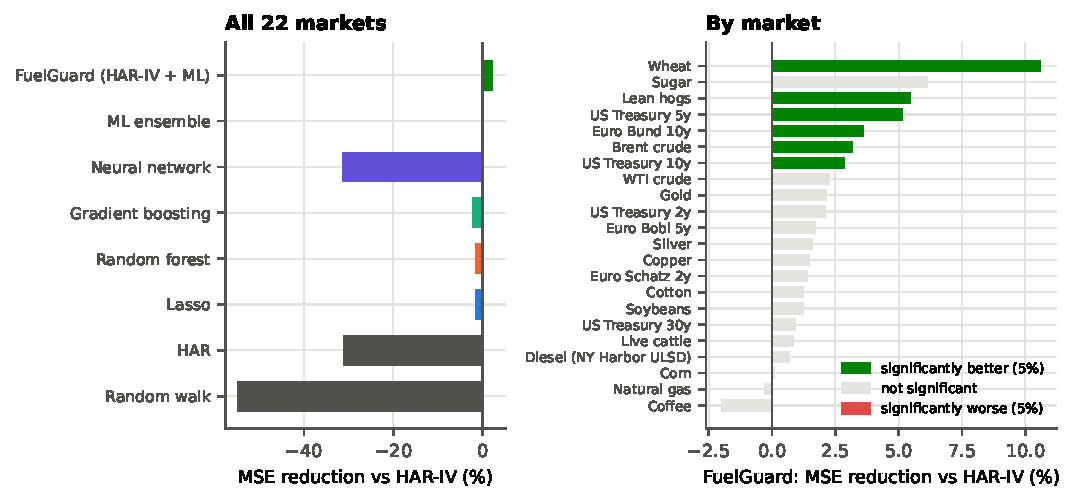
\includegraphics[width=\textwidth]{v2_fig_accuracy.pdf}
\caption{Left: MSE reduction against HAR-IV, all markets. Right: FuelGuard against HAR-IV by market; colour
indicates a Diebold--Mariano test at 5\%.}
\label{fig:accuracy}
\end{figure}

\paragraph{By market.} FuelGuard improves on HAR-IV in 20 of 22 markets, significantly in six (wheat, lean
hogs, Brent and three government bonds), and is never significantly worse (Figure~\ref{fig:accuracy}).
Gains are largest for wheat, sugar and lean hogs. For energy as a group the gain is
1.7\% ($p=0.04$); for diesel alone it is 0.7\% and not significant (Table~\ref{tab:diesel}): on its own
product, FuelGuard is as good as the best econometric benchmark, not clearly better.

\begin{table}[H]
\centering\small
\fittable{\tabdir/vol_diesel.tex}
\caption{Diesel (NY Harbor ULSD) only, 3\,724 out-of-sample days. DM test per market, Newey--West 21 lags.}
\label{tab:diesel}
\end{table}

\paragraph{What drives the forecasts.} Shuffling the implied-volatility features of the gradient-boosting
model raises its test error by 45\%, past realised volatility by 11\%, volume and curve by 4\%; smile,
variance risk premium, asymmetry and common risk factors each add 1--2\% (Figure~\ref{fig:importance}).
The economics is coherent: the option market's forecast is the main input, recent realised volatility
corrects it, and unusual volume (often news) signals that volatility is about to change.

\begin{figure}[t]
\centering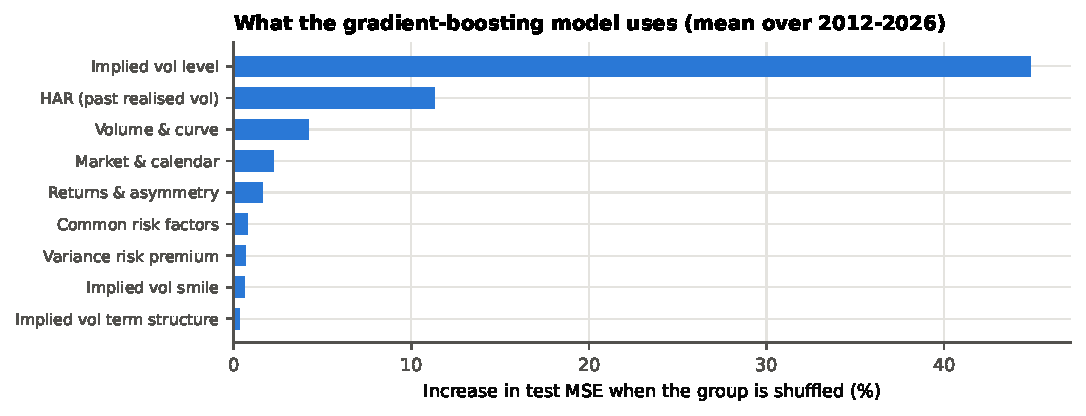
\includegraphics[width=0.9\textwidth]{v2_fig_importance.pdf}
\caption{Grouped permutation importance of gradient boosting on the test years: increase of test MSE when
all features of a group are shuffled together (mean over 2012--2026).}
\label{fig:importance}
\end{figure}

\subsection{Value for the haulier}

\begin{figure}[t]
\centering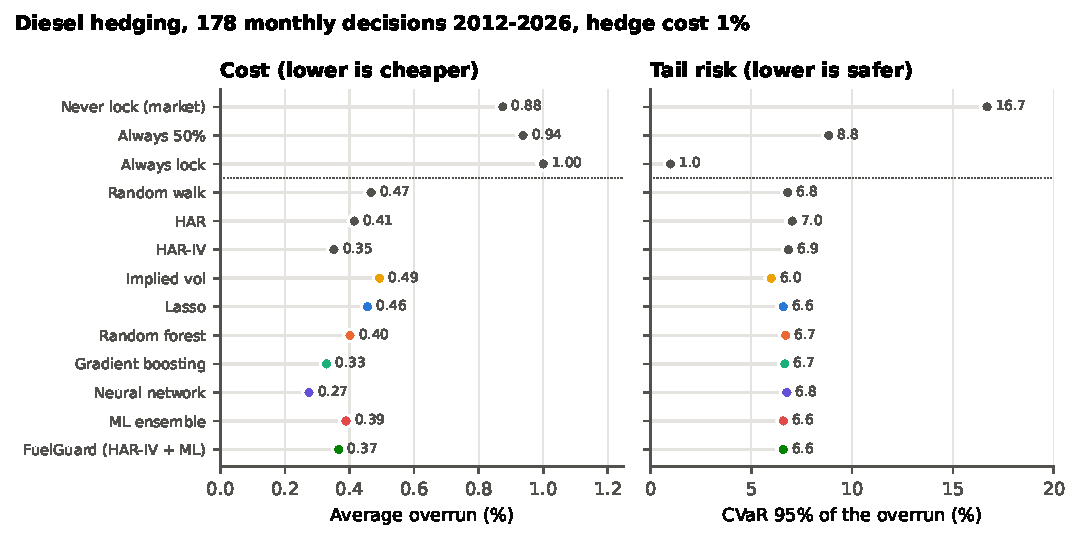
\includegraphics[width=\textwidth]{v2_fig_backtest.pdf}
\caption{Diesel hedging backtest. Each volatility forecast feeds the same rule (lock 100\% above the
historical 75th percentile of volatility, 50\% above the median). Overrun: monthly cost above the price
lockable at decision, with a 1\% hedging margin.}
\label{fig:backtest}
\end{figure}

\paragraph{Hedge ratio.} Figure~\ref{fig:backtest} and Table~\ref{tab:bt} (Appendix~\ref{app:additional})
evaluate 178 monthly decisions. Never hedging costs 0.88\% above the lockable price on average and 16.7\% in
the worst 5\% of months, about 2\,800~EUR more than the price that could have been fixed for our reference
firm. With FuelGuard, the firm hedges 40\% of months on average, its tail cost falls to \textbf{6.6\%}
(about 900~EUR) with only 8 months above a 5\% overrun instead of 38, and its average cost falls to 0.37\%,
saving about 900~EUR a year. A constant 50\% hedge achieves less (8.8\%) at a higher cost (0.94\%). The value
comes from \emph{conditioning the hedge on forecast risk}: all volatility forecasts, from the random walk to
FuelGuard, give tail costs between 6.0\% and 7.0\%, and the differences between them are within sampling
noise (the tail rests on 9 months).

\paragraph{95\% worst case.} The bound implied by FuelGuard's forecast averages 8.4\% above the lockable
price; it was exceeded in 14 of 178 months (7.9\% instead of 5\%; Kupiec $p=0.10$). All realised-volatility
models are slightly too optimistic (7--9\% breaches), because the Garman--Klass target ignores overnight
moves and the bound ignores fat tails; implied volatility, which includes the variance risk premium, has
correct coverage (5.6\%). A production version should scale the bound up by about 15\% or use implied
volatility as a floor.
